\documentclass{article}
\usepackage[margin=1in]{geometry}
\title{Minutes from 17 August}

\usepackage{float}
\usepackage{amsmath}
\usepackage{graphicx}
\usepackage{caption}
\usepackage{subcaption}
\usepackage{parskip}
\usepackage{url}

\begin{document}
	
\section{Frequency-smoothing encryption}
\begin{itemize}
	\item Original paper: Marie-Sarah Lacharit´e, Kenneth G. Paterson. \textbf{Frequency-smoothing encryption: preventing snapshot attacks on encrypted databases}
	
	\item The encryption scheme takes two stages: 1) smooth the frequency of the plaintexts given their distribution, 2) apply deterministic encryption to obtain the set of ciphertexts (homophones).
	
	\item But the process is done column by column in a database, the frequency smoothing procedure only smooth out the marginals, i.e. correlation between columns are still preserved. This means it is possible to use co-occurance information to attack the encrypted database (The attack is called counting attack in the searchable encryption setting. We cannot directly use the attack because the frequencies are `dispersed' by the FSE.).
\end{itemize}
	

\section{Attack setup}
\begin{itemize}
	\item Data used is the PUDF base data from first quarter of 2010 (\url{https://www.dshs.texas.gov/THCIC/Hospitals/Download.shtm}). This data set is publicly available unlike NIS data set. Since we only need to demonstrate feasibility of the attack, it suffices to use the earlier data set if we can find some correlated columns.
	
	\item The columns we attack on are risk mortality and illness severity (see manual in the repository).
	
	\item The frequency smoothing part of FSE has been re-implemented. We omit the deterministic encryption part of the scheme because it does no more than permuting the ciphertexts in our view. Our attack works regardless if DE has been applied.
\end{itemize}


\section{Correctness of implementation}
\begin{itemize}
	\item We use the same data as the base distribution, so the frequency smoothing algorithm will produce perfect uniformly distributed plaintexts (marginally).
	
	\item To verify that the implementation is correct we plot the histograms for the two columns:
	\begin{figure}[H]
		\centering
		\begin{subfigure}{.45\textwidth}
			\centering
			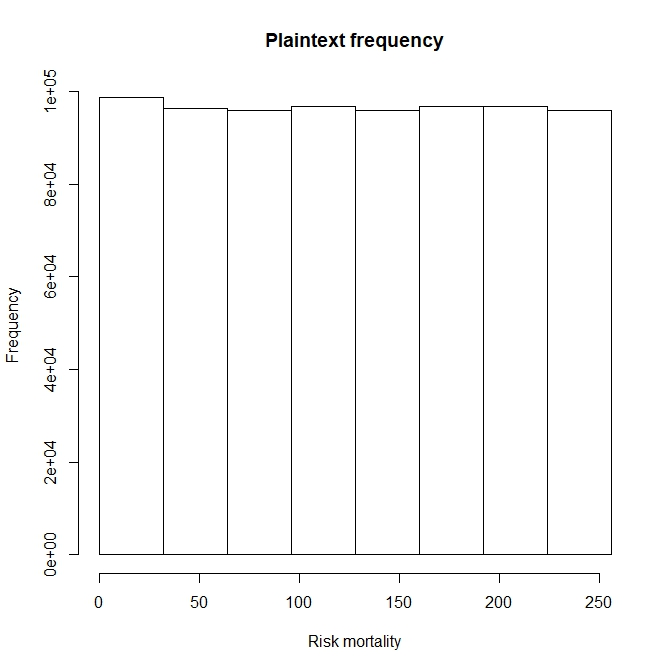
\includegraphics[width=1\linewidth]{./Img/img1.jpeg}
		\end{subfigure} %
		\begin{subfigure}{.45\textwidth}
			\centering
			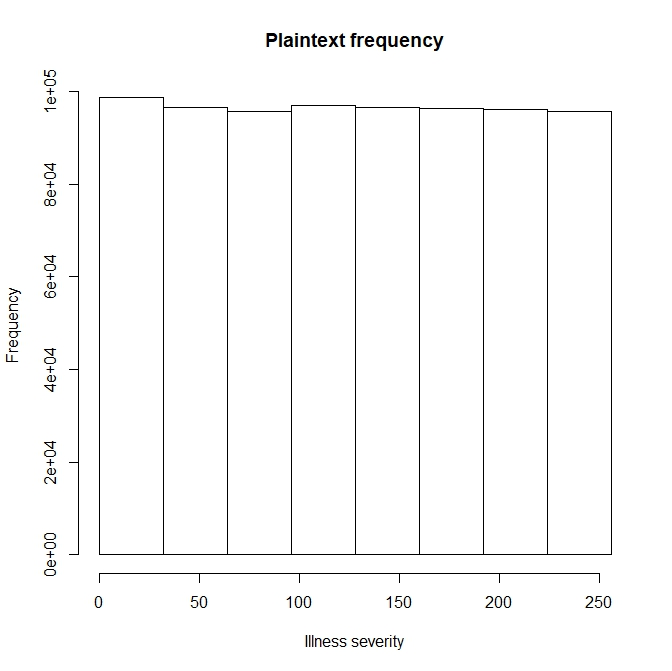
\includegraphics[width=1\linewidth]{./Img/img2.jpeg}
		\end{subfigure}
	\end{figure}
\end{itemize}


\section{The attack}
\subsection{Gather information}
\begin{itemize}
	\item There are 5 possible values for risk mortality and illness severity each, ranging from 0 to 4 respectively. We write 
	\begin{equation*}
		N(i,j) := | \{(x,y) \in DB\mid x = i, \ y = j\} |,
	\end{equation*}
	i.e. the number of occurrence which risk mortality is level $i$ and illness severity is level $j$. Due to correlation, $N(i, j)$ will be different for each $i$ and $j$.
	
	\item From our knowledge of the distribution of the attributes, we can also work out the size of plaintexts each of the attributes will take. This is simply $S(i) := 2^r * f(i)$, where $r$ is the number of bits used in the encoding, and $f(i)$ is the frequency of attribute $i$ (in a specific column). Therefore, for two columns, we can work out the size of the rectangle each pair of attributes will take (denoted by $S(i,j)$ in a similar way).
	
	\item In summary we will have:
	\begin{table}[H] \label{t1}
		\centering
		\begin{tabular}{|l|l|l|l|l|l|}
			\hline
			& 0    & 1      & 2      & 3     & 4     \\ \hline
			0 & 3144 & 0      & 0      & 0     & 0     \\ \hline
			1 & 0    & 280929 & 174412 & 24876 & 366   \\ \hline
			2 & 0    & 9692   & 76033  & 66129 & 2073  \\ \hline
			3 & 0    & 386    & 8373   & 65971 & 19157 \\ \hline
			4 & 0    & 130    & 164    & 6402  & 34857 \\ \hline
		\end{tabular}
		\caption{$N(i,j)$, row by column}
	\end{table}

	\begin{table}[H]
		\centering
		\begin{tabular}{|l|l|l|l|l|l|}
			\hline
			& 0   & 1     & 2     & 3    & 4    \\ \hline
			0 & 1   & 96    & 86    & 54   & 18   \\ \hline
			1 & 159 & 15264 & 13674 & 8586 & 2862 \\ \hline
			2 & 51  & 4896  & 4386  & 2754 & 918  \\ \hline
			3 & 31  & 2976  & 2666  & 1674 & 558  \\ \hline
			4 & 14  & 1344  & 1204  & 756  & 252  \\ \hline
		\end{tabular}
		\caption{$S(i,j)$, row by column}
	\end{table}
\end{itemize}


\subsection{Modelling co-occurrence}
Unlike the counting attack, the distribution of the counts on the co-occurrence matrix is much more complicated. So we want to work out the distributions first.

We know that attribute $(i, j)$ will be encrypted to a set of homophones, independent of other attributes, so we can model the distribution of the counts for each attribute separately. For attribute $(i,j)$, there are $N(i,j)$ encodings, and they are encoded independently and uniformly into $S(i,j)$ homophones. This is equivalent to the occupancy problem.

For each encoding of attribute $(i,j)$, the count on a particular homophone follows Bernoulli distribution with success rate $1 / S(i,j)$. Therefore with $N(i,j)$ iid copies of them, we obtain a binomial distribution 
\begin{equation*}
	\text{Bimon}\left(N(i,j), \frac{1}{S(i,j)}\right).
\end{equation*}

This distribution can be approximated by a normal distribution
\begin{equation*}
	\mathcal{N}\left(\frac{N(i,j)}{S(i,j)}, \frac{N(i,j)}{S(i,j)}\right).
\end{equation*}
since for large $S(i,j)$, $\frac{1}{S(i,j)} \approx 0$ so the variance is approximately equal to mean. This allows us to distinguish different attributes. Mean of the distributions on the counts are summarized in the following table:

\begin{table}[H] \label{t3}
	\centering
	\begin{tabular}{|l|l|l|l|l|l|}
		\hline
		& 0    & 1     & 2     & 3    & 4    \\ \hline
		0 & Deterministic      & 0    & 0    & 0   & 0   \\ \hline
		1 & 0  & 18.4 & 12.8   & 2.9  & 0.1 \\ \hline
		2 & 0  & 2.0  & 17.3   & 24.0 & 2.3  \\ \hline
		3 & 0  & 0.1  & 3.14   & 39.4 & 34.3  \\ \hline
		4 & 0  & 0.1  & 0.1    & 8.5  & 138.3  \\ \hline
	\end{tabular}
	\caption{$S(i,j)$}
\end{table}


For ease of visualisation, we obtain the counts on the co-occurrence without applying deterministic encryption for the first ten thousand rows in the database. The correlation can be easily recognised.
\begin{figure}[H] \label{plot}
	\centering
	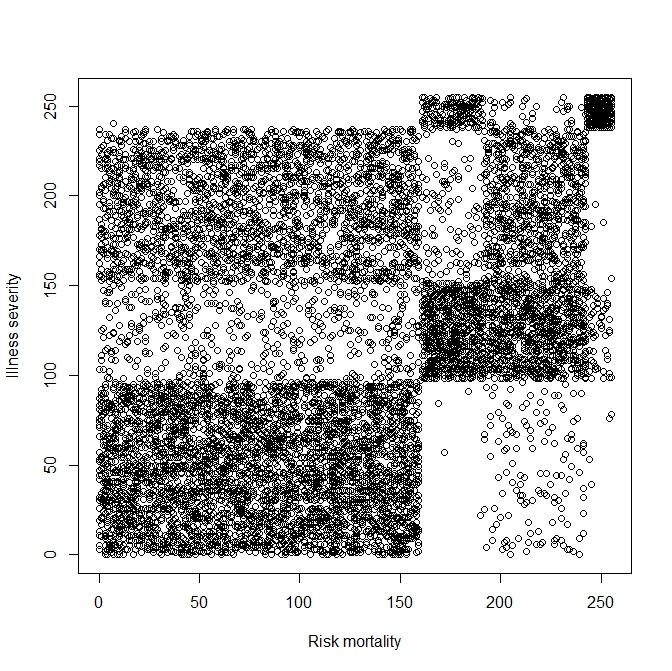
\includegraphics[width=0.6\linewidth]{./Img/img3.jpeg}
\end{figure}


\subsection{Executing the attack}
\subsection{An important remark}
To attack the co-occurrence matrix, we first identify the attribute we want to use. Ideally, the attribute should have mean very far from the rest, so the homophones can be easily identified. One thing to note is that each time we successfully recover some attribute $(i,j)$, we actually get
\begin{equation*}
	\{\text{encodings of } i\} = \cup \{ \Pi_{1} (a,b) \mid \text{we belive } (a,b) \text{ is homophone of } (i,j)\}
\end{equation*}
likewise for encodings of $j$ (this can be put more formally but let's leave it like this for now).

So for instance, if we manage to recover the top right block as attribute $(i,j)$ (in reality it will not be a block due to application of DE), we also know that the vertical and horizontal strip associated to it are that of $i$ and $j$ respectively.


\subsection{Example of recovery attacks}
We first spot that attribute $(0,0)$ has only one homophone, this is because there is only one homophone in each dimension. We check from table \ref{t1} that it has count 3144, and the next highest (in terms of distribution) has mean of 138.3. So we can safely assign the encoding that has count of over 300 say, to attribute $(0,0)$ if our prior knowledge is not exact. In case of exact knowledge, we simply choose the encoding that has count 3144 and make the conclusion.

Since attribute $(0,0)$ is a singleton and the corresponding rows and columns in $N(i,j)$ have zero everywhere else. We cannot obtain more information from this attribute.

We then look at the next attribute that has the highest mean. That is attribute $(4,4)$. The next highest mean int he table is 39.4 which is much smaller, so we can set all encodings with count greater than 103.0 (3 standard deviation less than the mean) to be homophones of attribute $(4,4)$. In the experiment, the accuracy of recovery is 100\%.

We then can look at rows and columns corresponds to attribute $(4,4)$ and identify homophones in those restricted domains. For example, the last column of \ref{t3} corresponds to the top horizontal strip of figure \ref{plot}, and we can identify attribute $(3,4)$ from the rest using the same method.


\end{document}